% !TeX encoding = UTF-8
% !TeX program = pdfLaTeX
% !TeX root = markertracker.tex
% !TeX spellcheck = en_US
\documentclass[10pt,a4paper]{article}
\usepackage[utf8]{inputenc}
\usepackage[T1]{fontenc}
\usepackage{amsmath}
\usepackage{amsfonts}
\usepackage{amssymb}
\usepackage{todonotes}
\usepackage{placeins}
\begin{document}


\section{Marker tracker}

A few notes on the marker tractor (indoor
gps system for Robdab.
The system is based on the Fourier transform
for detecting square waves (see figure \ref{figSquareWave}).
The square
eave is observed when going around the
center of the marker.
\begin{figure}
\centering
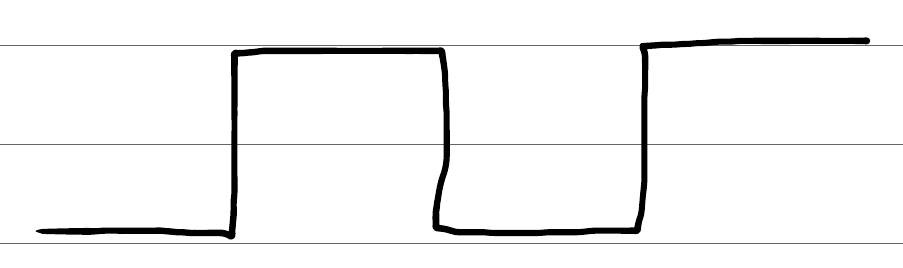
\includegraphics[width=0.6\linewidth]{pic/squarewave.png}
\caption{Example square wave.}
\label{figSquareWave}
\end{figure}

The square wave can be represented by
a fourier series on the form
\begin{align}
f\left( x\right) =\sum ^{\infty }_{k=1}\dfrac {\sin \left( kx\right) }{k}
\end{align}
When searching for the marker, only the
two first terms in the Fourier expansion
is taken into account 
\begin{align}
f\left( x\right) =\sin \left( x\right) +\dfrac {1}{3}\sin \left( 3x\right) +\ldots
\end{align}
The first term is used to determine the
strength and orientation of the marker
the second term is used to measure
the quality of the found marks.
If the marker is rotated, it gives a
shift in the square wane
\begin{align}
f\left( x+x_{0}\right) =\sin \left( x+x_{0}\right) +\dfrac {1}{3}\sin \left( 3x+3x_{0}\right) +\ldots
\end{align}
notice how the phase shift is three
time, larger in the second term than in
the first term.This property is used to
determine the quality of a found marker.
The ideal marker would look like
shown in figure \ref{figIdealSineDecomposition}.

\begin{figure}[ht]
\centering
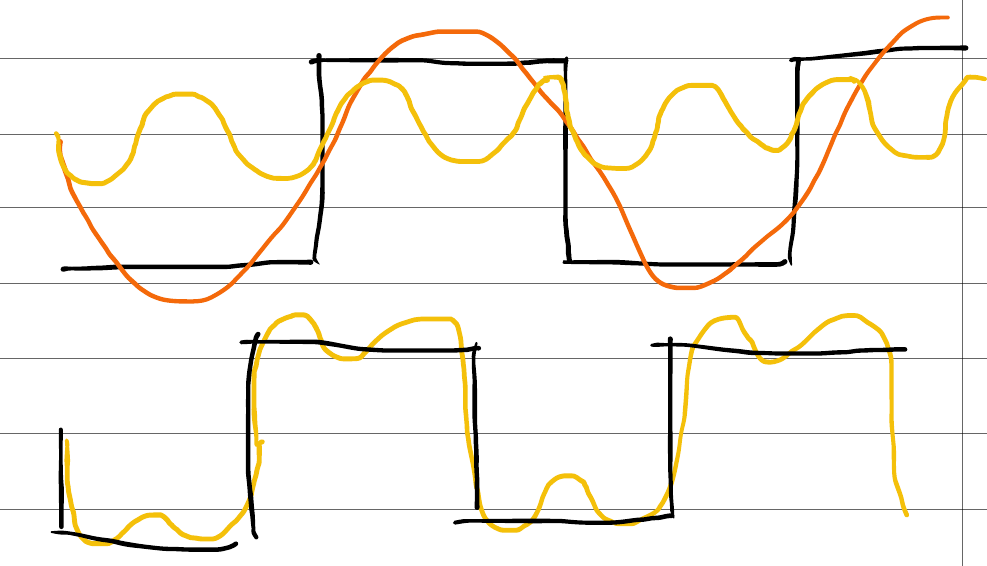
\includegraphics[width=0.6\linewidth]{pic/idealmarkerwaveform.png}
\caption{Ideal marker waveform decomposed into sines.}
\label{figIdealSineDecomposition}
\end{figure}

If the two sine waves are out of phase, the
reconstructed wave can look like.
\missingfigure{}
This effect is used to evaluate the quality
of the detected marker.

The marker can have different orders / appearances,
The order is the number of repetitions of a
square wave that the marker is constructed of,

\begin{figure}[ht]
\centering
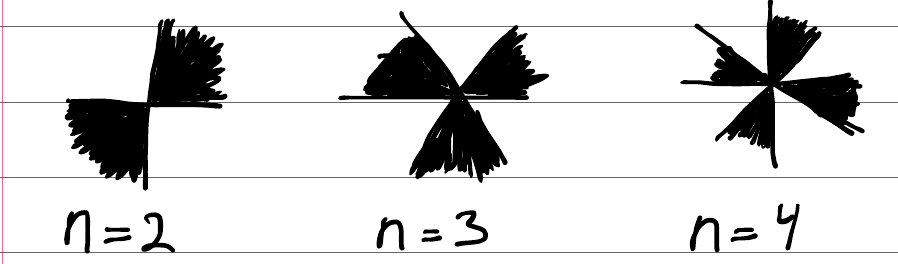
\includegraphics[width=0.8\linewidth]{pic/differentmarkerorders.png}
\caption{Different marker orders.}
\label{figOrdersOfMarkers}
\end{figure}

The examples of markers three different orders
are shown above To add an orientation to
the marker one of the black regions are
removed

\begin{figure}[ht]
\centering
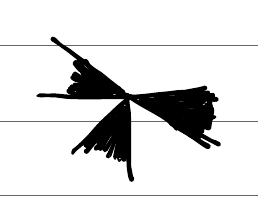
\includegraphics[width=0.3\linewidth]{pic/markerwithindicatedorientation.png}
\caption{}
\label{fig}
\end{figure}

The con of removing a part of the pattern is
a weaker response, The tracker determines possible
orientations based on the detected phase of the
marker, Then is the color of each region
measured and the brightest region determines
the orientation.


\end{document}